\documentclass[a4paper,12pt]{article}

% Самые необходимые пакеты
\usepackage[T2A]{fontenc}
\usepackage[utf8]{inputenc}
\usepackage[russian]{babel}
\usepackage{geometry}
\usepackage{amsmath}
\usepackage{graphicx}
\usepackage{float} 

% Настройка геометрии
\geometry{left=1.5cm, right=2cm, bottom=2cm, top=2cm}

\begin{document}
	
	% Титульный лист
	\begin{titlepage}
		\centering
		\vspace*{1cm}
		
		% Министерство
		{\small
			Министерство науки и высшего образования Российской Федерации\\
			Федеральное государственное автономное образовательное учреждение\\
			высшего образования\\
			«Национальный исследовательский университет ИТМО»\\
		}
		
		\vspace{2cm}
		
		% Факультет
		{\large
			Факультет систем управления и робототехники\\
		}
		
		\vspace{3cm}
		
		% Основной заголовок
		{\Huge\bfseries
			ОТЧЕТ\\
		}
		\vspace{0.5cm}
		{\LARGE\bfseries
			о лабораторной работе №1\\
		}
		
		\vspace{1cm}
		
		% Дисциплина и тема
		{\Large
			По дисциплине: «Линейные системы автоматического управления»\\
			\vspace{0.5cm}
			Тема: «Формы представления линейных динамических систем»\\
		}
		
		\vspace{3cm}
		
		% Информация о студенте и преподавателях
		\begin{minipage}{0.4\textwidth}
			\raggedright
			{\large
				Студент:\\
			}
			Охрименко Е. Д.\\
			Поток: 1.1.3\\
			Вариант: 17\\
		\end{minipage}
		\hfill
		\begin{minipage}{0.4\textwidth}
			\raggedleft
			{\large
				Преподаватель:\\
			}
			Пашенко А. В.\\
		\end{minipage}
		
		\vfill
		
		% Город и год
		{\large
			Санкт-Петербург\\
			2025\\
		}
		
	\end{titlepage}
	
	\newpage
	\tableofcontents
	\newpage
	
	\section{Задание. Одноканальная система в форме вход-выход}
	
	В этом задании мне нужно:
	
	\begin{itemize}
		
		\item Рассмотреть математическую модель в форме дифференциального уравнения: 
		
		\[\dddot{y} + a_2\ddot{y} + a_1\dot{y} + a_0y = b_2\ddot{u} + b_1\dot{u} + b_0u\]
		
		\item Построить структурную схему системы с использованием блоков элементарных операций (интеграторов, сумматоров).
		
		\item Выполнить моделирование при \(u(t) = 1\), \(\ddot{y}(0) = \dot{y}(0) = y(0) = 0\).
		
		\item Записать математическую модель системы, привести структурную схему cистемы и графики \(y(t)\) и \(u(t)\).
		
	\end{itemize}
	
	
	
	\subsection{Математическая модель системы}

	Запишу уравнение:
	
	\[\dddot{y} + a_2\ddot{y} + a_1\dot{y} + a_0y = b_2\ddot{u} + b_1\dot{u} + b_0u\]
	
	Применю дифференциальный оператор:
	
	\[y \cdot p^3 + a_2 y \cdot p^2+ a_1 y \cdot p + a_0 y = b_2 u \cdot p^2  + b_1 u \cdot p + b_0u\]
	
	Поделю на \(p^3\):
	
	\[y + a_2 y \cdot \frac{1}{p}  + a_1 y \cdot\frac{1}{p^2} + a_0 y \cdot \frac{1}{p^3} = b_2 u \cdot \frac{1}{p}  + b_1 u \frac{1}{p^2} + b_0u \frac{1}{p^3}\]
	
	Приведу подобные слагаемые и выражу \(y\):
	
	\[
		y = (b_2 u - a_2 y) \cdot \frac{1}{p} + (b_1 u - a_1 y) \cdot \frac{1}{p^2} + (b_0 u - a_0 y) \cdot \frac{1}{p^3} 
	\]
	
	Затем вынесу общие множители за скобки
	
	\[
	y = \frac{1}{p} \cdot \left( b_2 u - a_2 y + \frac{1}{p} \cdot \left( b_1 u - a_1 y + \frac{1}{p} \cdot (b_0 u - a_0 y) \right) \right)
	\]
	
	Подставлю параметры из моего варианта и получу: 
	
	\[
	y = \frac{1}{p} \cdot \left( 12 u - 8 y + \frac{1}{p} \cdot \left( 24 u - 19 y + \frac{1}{p} \cdot (42 u - 12 y) \right) \right)
	\]
	
	В таком виде удобно воспринимать систему, чтобы собрать структурную схему.
	
	\subsection{Структурная схема системы}
	
	Построю схему по получившийся математической модели в \texttt{Matlab Simulink}.
	
	\begin{figure}[H]
		\centering
		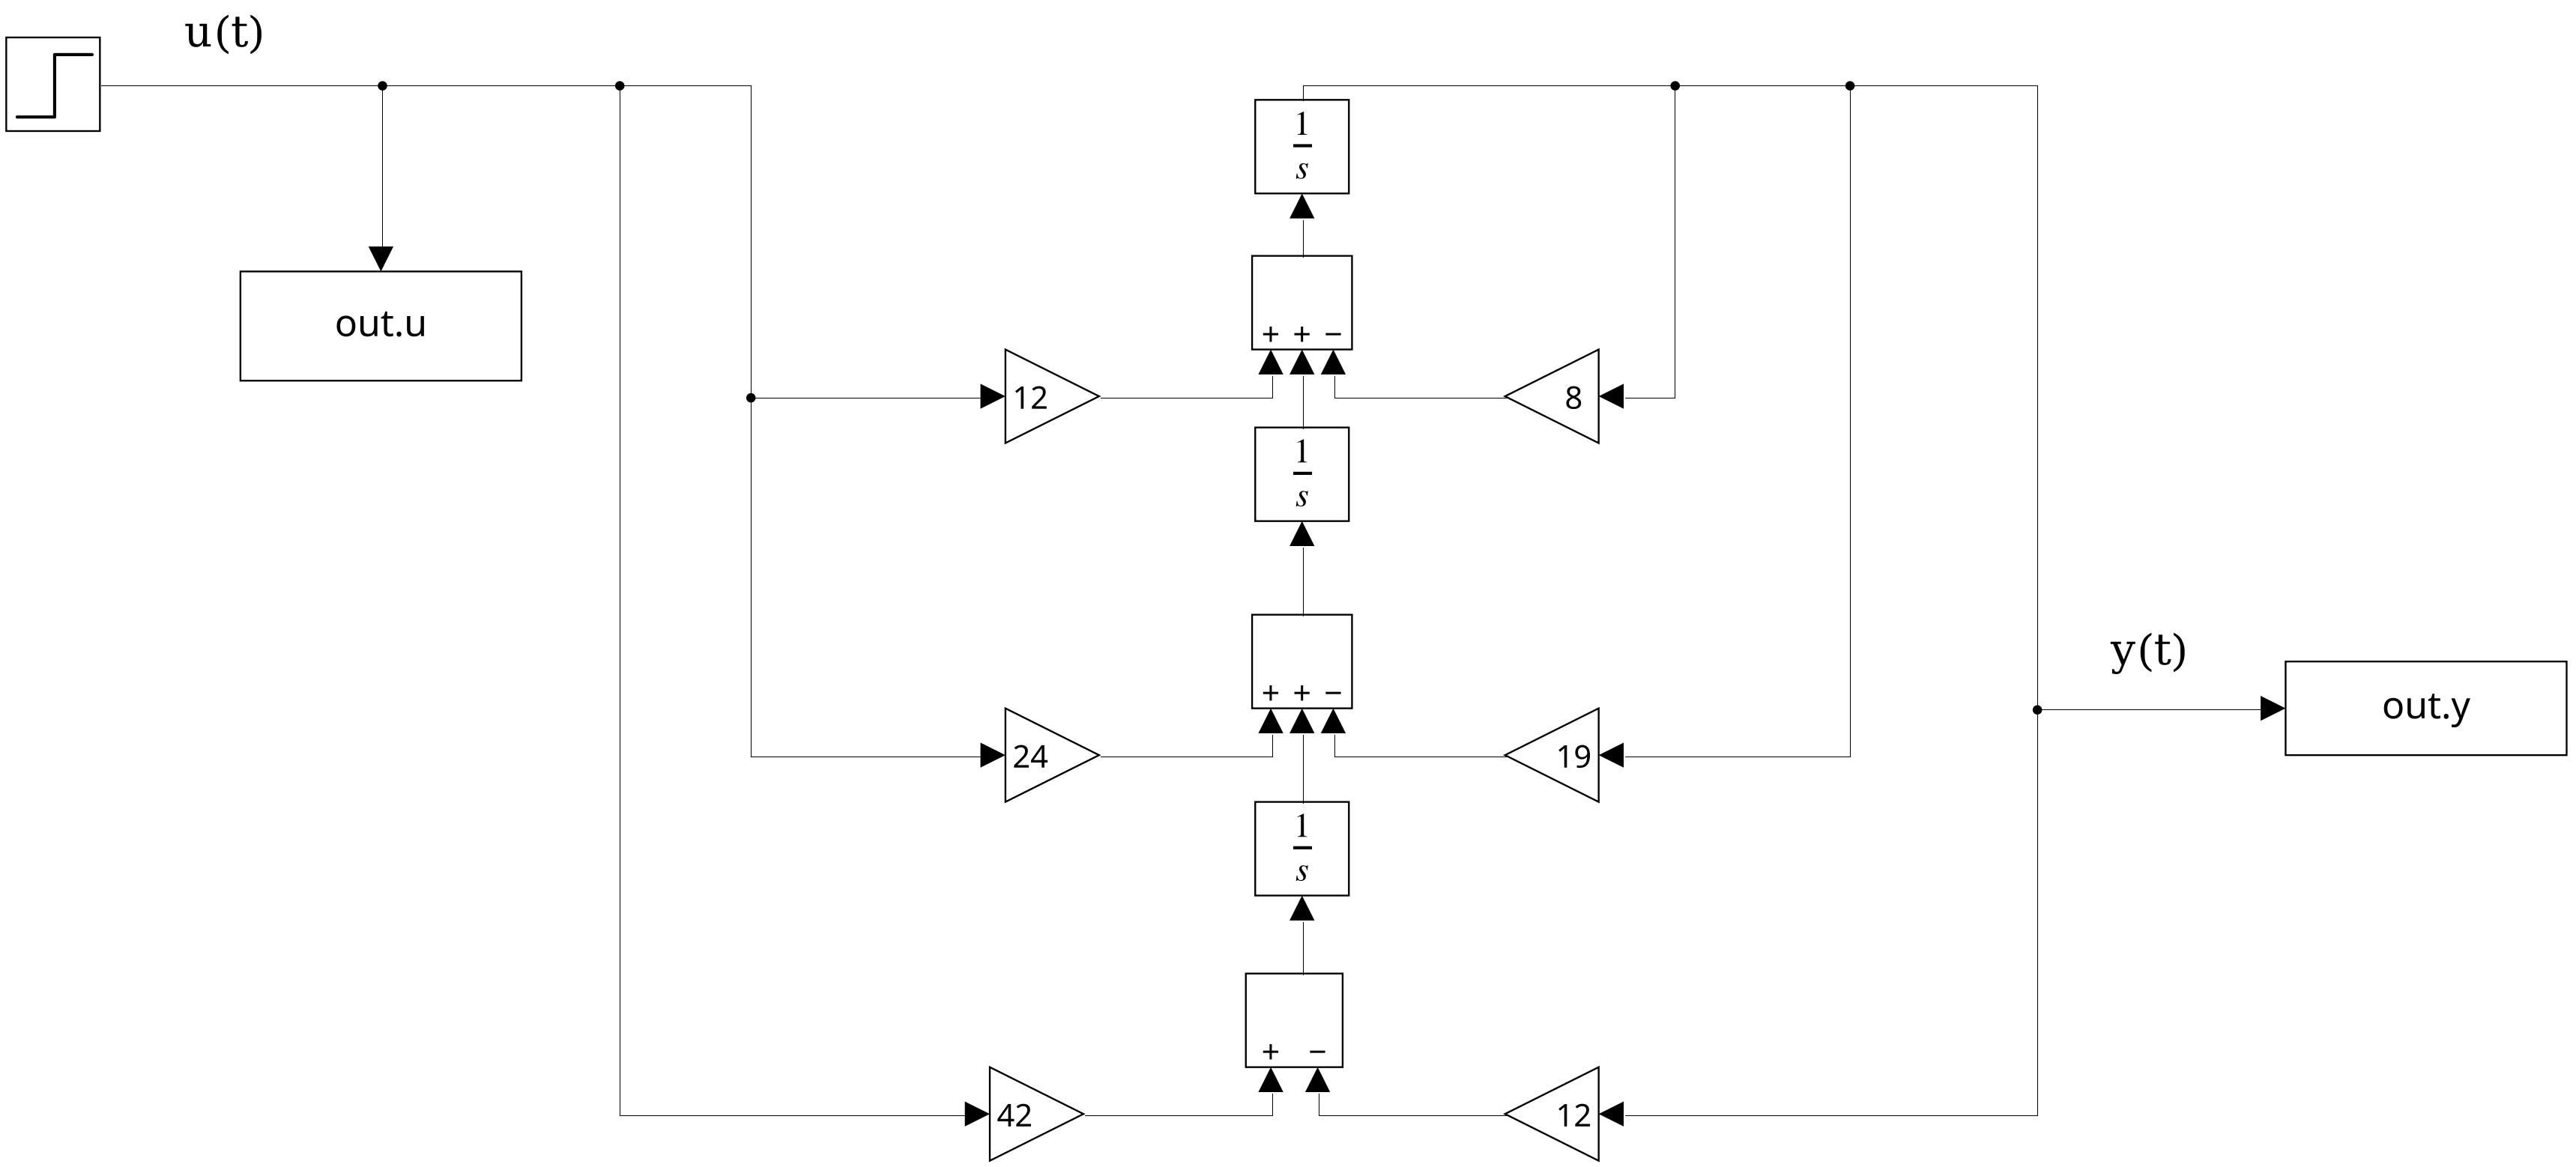
\includegraphics[width=1\textwidth]{../images/task1/model.png}
		\caption{Структурная схема системы}
	\end{figure}
	
	\subsection{Графики входа и выхода}
	
	Подам на вход 1 при помощи блока \texttt{Step}. Получится скачок от 0 до единицы в момент времени \(t = 0.0\).
	
	\begin{figure}[H]
		\centering
		
\includegraphics[width=0.9\textwidth]{../images/task1/u.png}
		\caption{Входной сигнал \(u(t)\)}
	\end{figure}
	
	На выходе системы получу переходный процесс \(y(t)\), который показывает реакцию системы на единичное ступенчатое воздействие. Как видно из графика, система выходит на установившееся значение \(y(\infty) = 3.5\).
	
	\begin{figure}[H]
		\centering
		
\includegraphics[width=0.9\textwidth]{../images/task1/y.png}
		\caption{Выходной сигнал \(y(t)\)}
	\end{figure}
	
	Посчитаю, на какое значение \textit{должна} выйти система. Запишу дифференциальное уравнение системы:
	
	\[\dddot{y} + 8\ddot{y} + 19\dot{y} + 12y = 12\ddot{u} +24\dot{u} + 42u\]
	
	Применю дифференциальный оператор:
	
	\[y \cdot p^3 + 8 y \cdot p^2+ 19  y \cdot p + 12 y = 12 u \cdot p^2  + 24 u \cdot p + 42u\]
	
	Запишу передаточную функцию системы:
	
	\[
	y = \underbrace{\frac{12 p^2 + 24 p + 42}{p^3 + 8 p^2 + 19 p + 12}}_{\textstyle W(p)} \cdot u
	\]


	Для единичного ступенчатого воздействия $u(t) = 1(t)$ установившееся значение:
	
	\[
	y(\infty) = \lim_{p \to 0} W(p) = \frac{42}{12} = 3.5
	\]
	
	\textbf{Итог: }Теоретическое значение сошлось с практическим, значит схема построена верно.
	
	\newpage
	
	\section{Задание. Переход от формы вход-выход к форме вход-состояние-выход}
	
	Для системы, заданной дифференциальным уравнением
	\[
	\dddot{y} + a_2 \ddot{y} + a_1 \dot{y} + a_0 y = b_2 \ddot{u} + b_1 \dot{u} + b_0 u,
	\]
	необходимо:
	
	\begin{itemize}
		\item Определить передаточную функцию \(W(p)\).
		\item Построить модели вход-состояние-выход в канонических управляемой, наблюдаемой и диагональной формах.
		\item Построить структурные схемы моделей с использованием элементарных блоков (интеграторы, сумматоры) и явно обозначенными состояниями.
		\item Выполнить моделирование при \(u(t) = 1\), \(y(0) = \dot{y}(0) = \ddot{y}(0) = 0\) и сравнить графики выходов всех моделей.
	\end{itemize}
	
	\subsection{Математические модели системы}
	
	Приведу дифференциальное уравнение 
	
		\[\dddot{y} + a_2\ddot{y} + a_1\dot{y} + a_0y = b_2\ddot{u} + b_1\dot{u} + b_0u\]
	
	к различным каноническим формам.
	
	\subsubsection{Каноническая управляемая форма}
	
	В матричном виде:
	
	\[
	\dot{x} = 
	\begin{bmatrix}
		0 & 1 & 0 \\
		0 & 0 & 1 \\
		-a_0 & -a_1 & -a_2
	\end{bmatrix} \cdot 
	\begin{bmatrix}
		x_1 \\x_2\\x_3\\
	\end{bmatrix} + 
	\begin{bmatrix}
		0 \\ 0 \\ 1
	\end{bmatrix} u,
	\quad
	y = [b_0 \quad b_1 \quad b_2] \cdot 
	\begin{bmatrix}
		x_1 \\x_2\\x_3\\
	\end{bmatrix}
	\]
	
	В соответствии с моим вариантом: 

	\[
	\dot{x} = 
	\begin{bmatrix}
		0 & 1 & 0 \\
		0 & 0 & 1 \\
		-12 & -19 & -8
	\end{bmatrix} \cdot 
	\begin{bmatrix}
		x_1 \\x_2\\x_3\\
	\end{bmatrix} + 
	\begin{bmatrix}
		0 \\ 0 \\ 1
	\end{bmatrix} u,
	\quad
	y = [42 \quad 24 \quad 12] \cdot 
	\begin{bmatrix}
		x_1 \\x_2\\x_3\\
	\end{bmatrix}
	\]
	
	Запишу в виде системы дифференциальных уравнений:
	
	\[
	\begin{cases}
		\dot{x}_1 = x_2 \\[6pt]
		\dot{x}_2 = x_3 \\[6pt]
		\dot{x}_3 = -12 x_1 - 19 x_2 - 8 x_3 + u \\[6pt]
		y = 42 x_1 + 24 x_2 + 12 x_3
	\end{cases}
	\]
	
	\subsubsection{Каноническая наблюдаемая форма}
	
	В матричном виде:
	
	\[
	\dot{x} = 
	\begin{bmatrix}
		0 & 0 & -a_0 \\
		1 & 0 & -a_1 \\
		0 & 1 & -a_2
	\end{bmatrix} 
	\begin{bmatrix}
		x_1 \\ x_2 \\ x_3
	\end{bmatrix} 
	+ 
	\begin{bmatrix}
		b_0 \\ b_1 \\ b_2
	\end{bmatrix} u,
	\quad
	y = 
	\begin{bmatrix}
		0 & 0 & 1
	\end{bmatrix}
	\begin{bmatrix}
		x_1 \\ x_2 \\ x_3
	\end{bmatrix}
	\]
	
	В соответствии с моим вариантом: 
	
	\[
	\dot{x} = 
	\begin{bmatrix}
		0 & 0 & -12 \\
		1 & 0 & -19 \\
		0 & 1 & -8
	\end{bmatrix} 
	\begin{bmatrix}
		x_1 \\ x_2 \\ x_3
	\end{bmatrix} 
	+ 
	\begin{bmatrix}
		42 \\ 24 \\ 12
	\end{bmatrix} u,
	\quad
	y = 
	\begin{bmatrix}
		0 & 0 & 1
	\end{bmatrix}
	\begin{bmatrix}
		x_1 \\ x_2 \\ x_3
	\end{bmatrix}
	\]
	
	Запишу в виде системы дифференциальных уравнений:
	
	\[
	\begin{cases}
		\dot{x}_1 = -12 x_3 + 42 u \\[6pt]
		\dot{x}_2 = x_1 - 19 x_3 + 24 u \\[6pt]
		\dot{x}_3 = x_2 - 8 x_3 + 12 u \\[6pt]
		y = x_3
	\end{cases}
	\]
	
	\subsubsection{Каноническая диагональная форма}
	
	Запишу в общем виде.
	
	Передаточная функция:
	\[
	W(p) = \frac{b_2 p^2 + b_1 p + b_0}{p^3 + a_2 p^2 + a_1 p + a_0} = 
	\frac{\beta_1 \gamma_1}{p - \lambda_1} + \frac{\beta_2 \gamma_2}{p - \lambda_2} + \frac{\beta_3 \gamma_3}{p - \lambda_3}.
	\]
	
	Состояния и уравнения системы:
	
	\[
	\dot{x} = 
	\begin{bmatrix}
		\lambda_1 & 0 & 0 \\
		0 & \lambda_2 & 0 \\
		0 & 0 & \lambda_3
	\end{bmatrix} x +
	\begin{bmatrix}
		\beta_1 \\ \beta_2 \\ \beta_3
	\end{bmatrix} u,
	\quad
	y = 
	\begin{bmatrix}
		\gamma_1 & \gamma_2 & \gamma_3
	\end{bmatrix} x,
	\quad
	x = \begin{bmatrix} x_1 \\ x_2 \\ x_3 \end{bmatrix}.
	\]
	
	Согласно моему варианту: 
	
	\[
	W(p) = \frac{12p^2 + 24 p + 42}{p^3 + 8 p^2 + 19 p + 12} 
	\]
	
	Теперь, при помощи функции \texttt{residue()} получу значения \(\lambda_i\) и \(\beta_i\gamma_i\). Получится:
	
	\[
	W(p) = \frac{12p^2 + 24 p + 42}{p^3 + 8 p^2 + 19 p + 12}  = 
	\frac{46}{p + 4} - \frac{39}{p + 3} + \frac{5}{p + 1}.
	\] 
	
	Определю \(\gamma_i = 1\) для удобства и запишу диагнальную форму системы:
	
	\[
	\dot{x} = 
	\begin{bmatrix}
		-4 & 0 & 0 \\
		0 & -3 & 0 \\
		0 & 0 & -1
	\end{bmatrix} x +
	\begin{bmatrix}
		46 \\ -39 \\ 5
	\end{bmatrix} u,
	\quad
	y = 
	\begin{bmatrix}
		1 & 1 & 1
	\end{bmatrix} x,
	\quad
	x = \begin{bmatrix} x_1 \\ x_2 \\ x_3 \end{bmatrix}.
	\]
	
	\newpage
	Запишу в виде системы дифференциальных уравнений:
	
	\[
	\begin{cases}
		\dot{x}_1 = -4 x_1 + 46 u \\[6pt]
		\dot{x}_2 = -3 x_2 - 39 u \\[6pt]
		\dot{x}_3 = -1 x_3 + 5 u \\[6pt]
		y = x_1 + x_2 + x_3
	\end{cases}
	\]
		
	\subsection{Структурные схемы системы}
	
	Построю структурные схемы системы, также явно подпишу каналы, соответствующие компонентам векторов состояния \(x\).
	
	\begin{figure}[H]
		\centering
		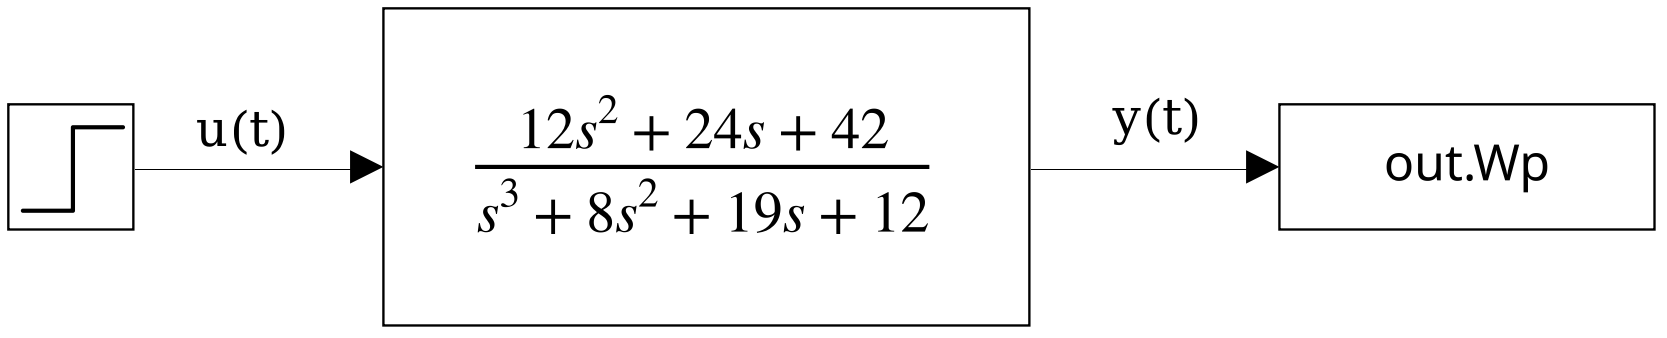
\includegraphics[width=0.6\textwidth]{../images/task2/model_Wp.png}
		\caption{Сруктурная схема системы при помощи блока \texttt{Transfer FCN}}
	\end{figure}
	
	\subsubsection{Каноническая управляемая форма}
	
	\begin{figure}[H]
		\centering
		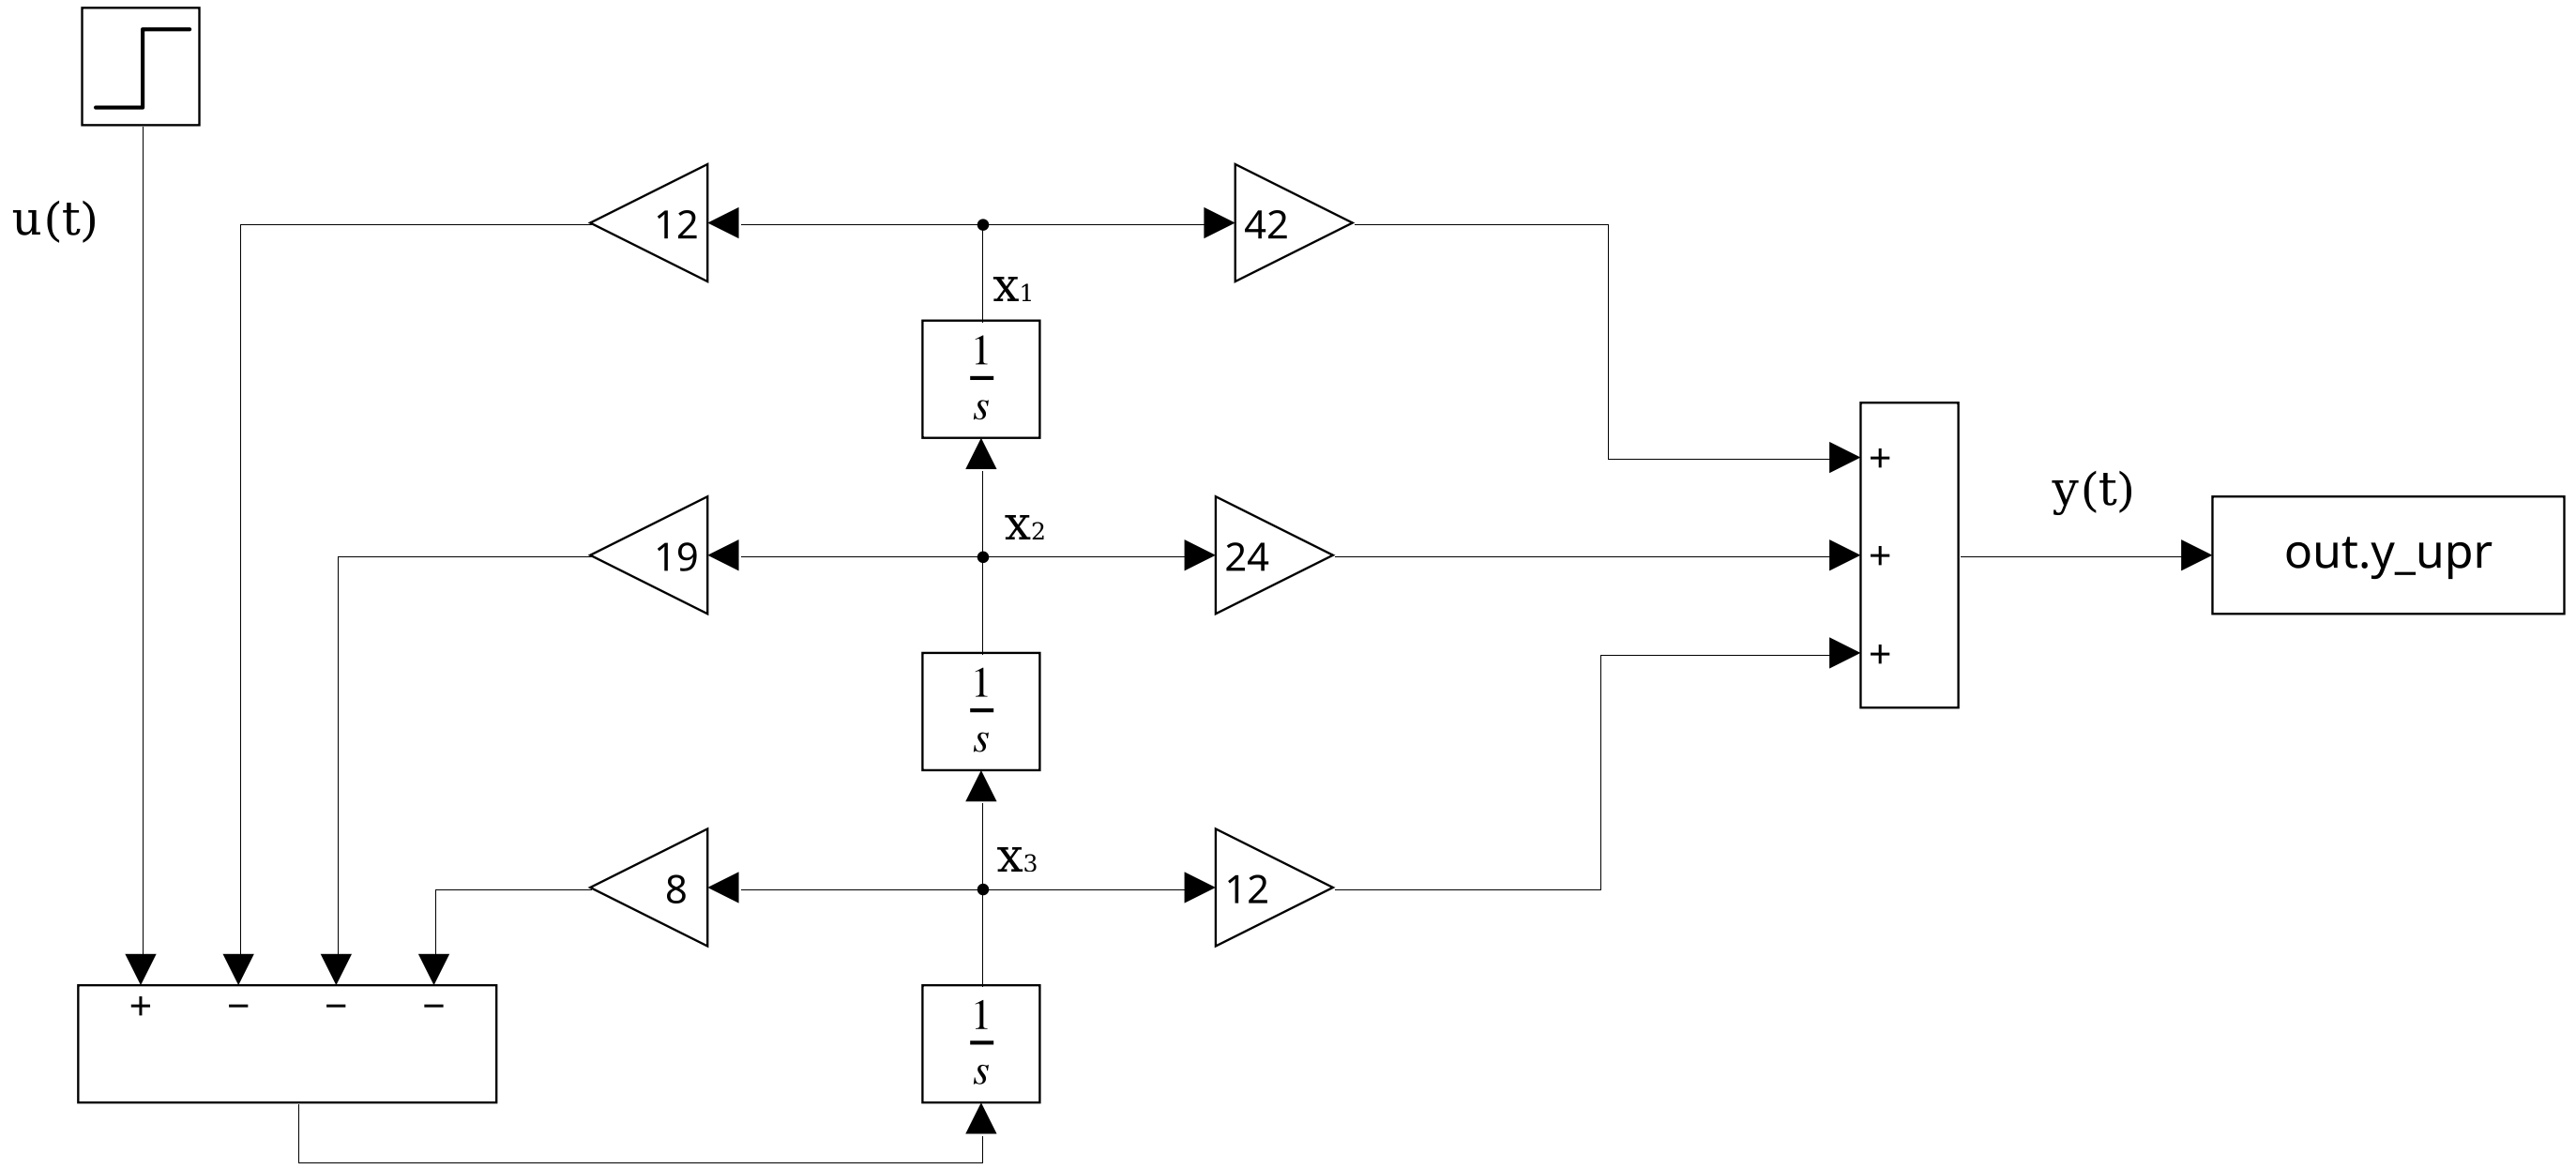
\includegraphics[width=1\textwidth]{../images/task2/model_upr.png}
		\caption{Сруктурная схема системы в канонической управляемой форме}
	\end{figure}
	
	\subsubsection{Каноническая наблюдаемая форма}
	
	\begin{figure}[H]
		\centering
		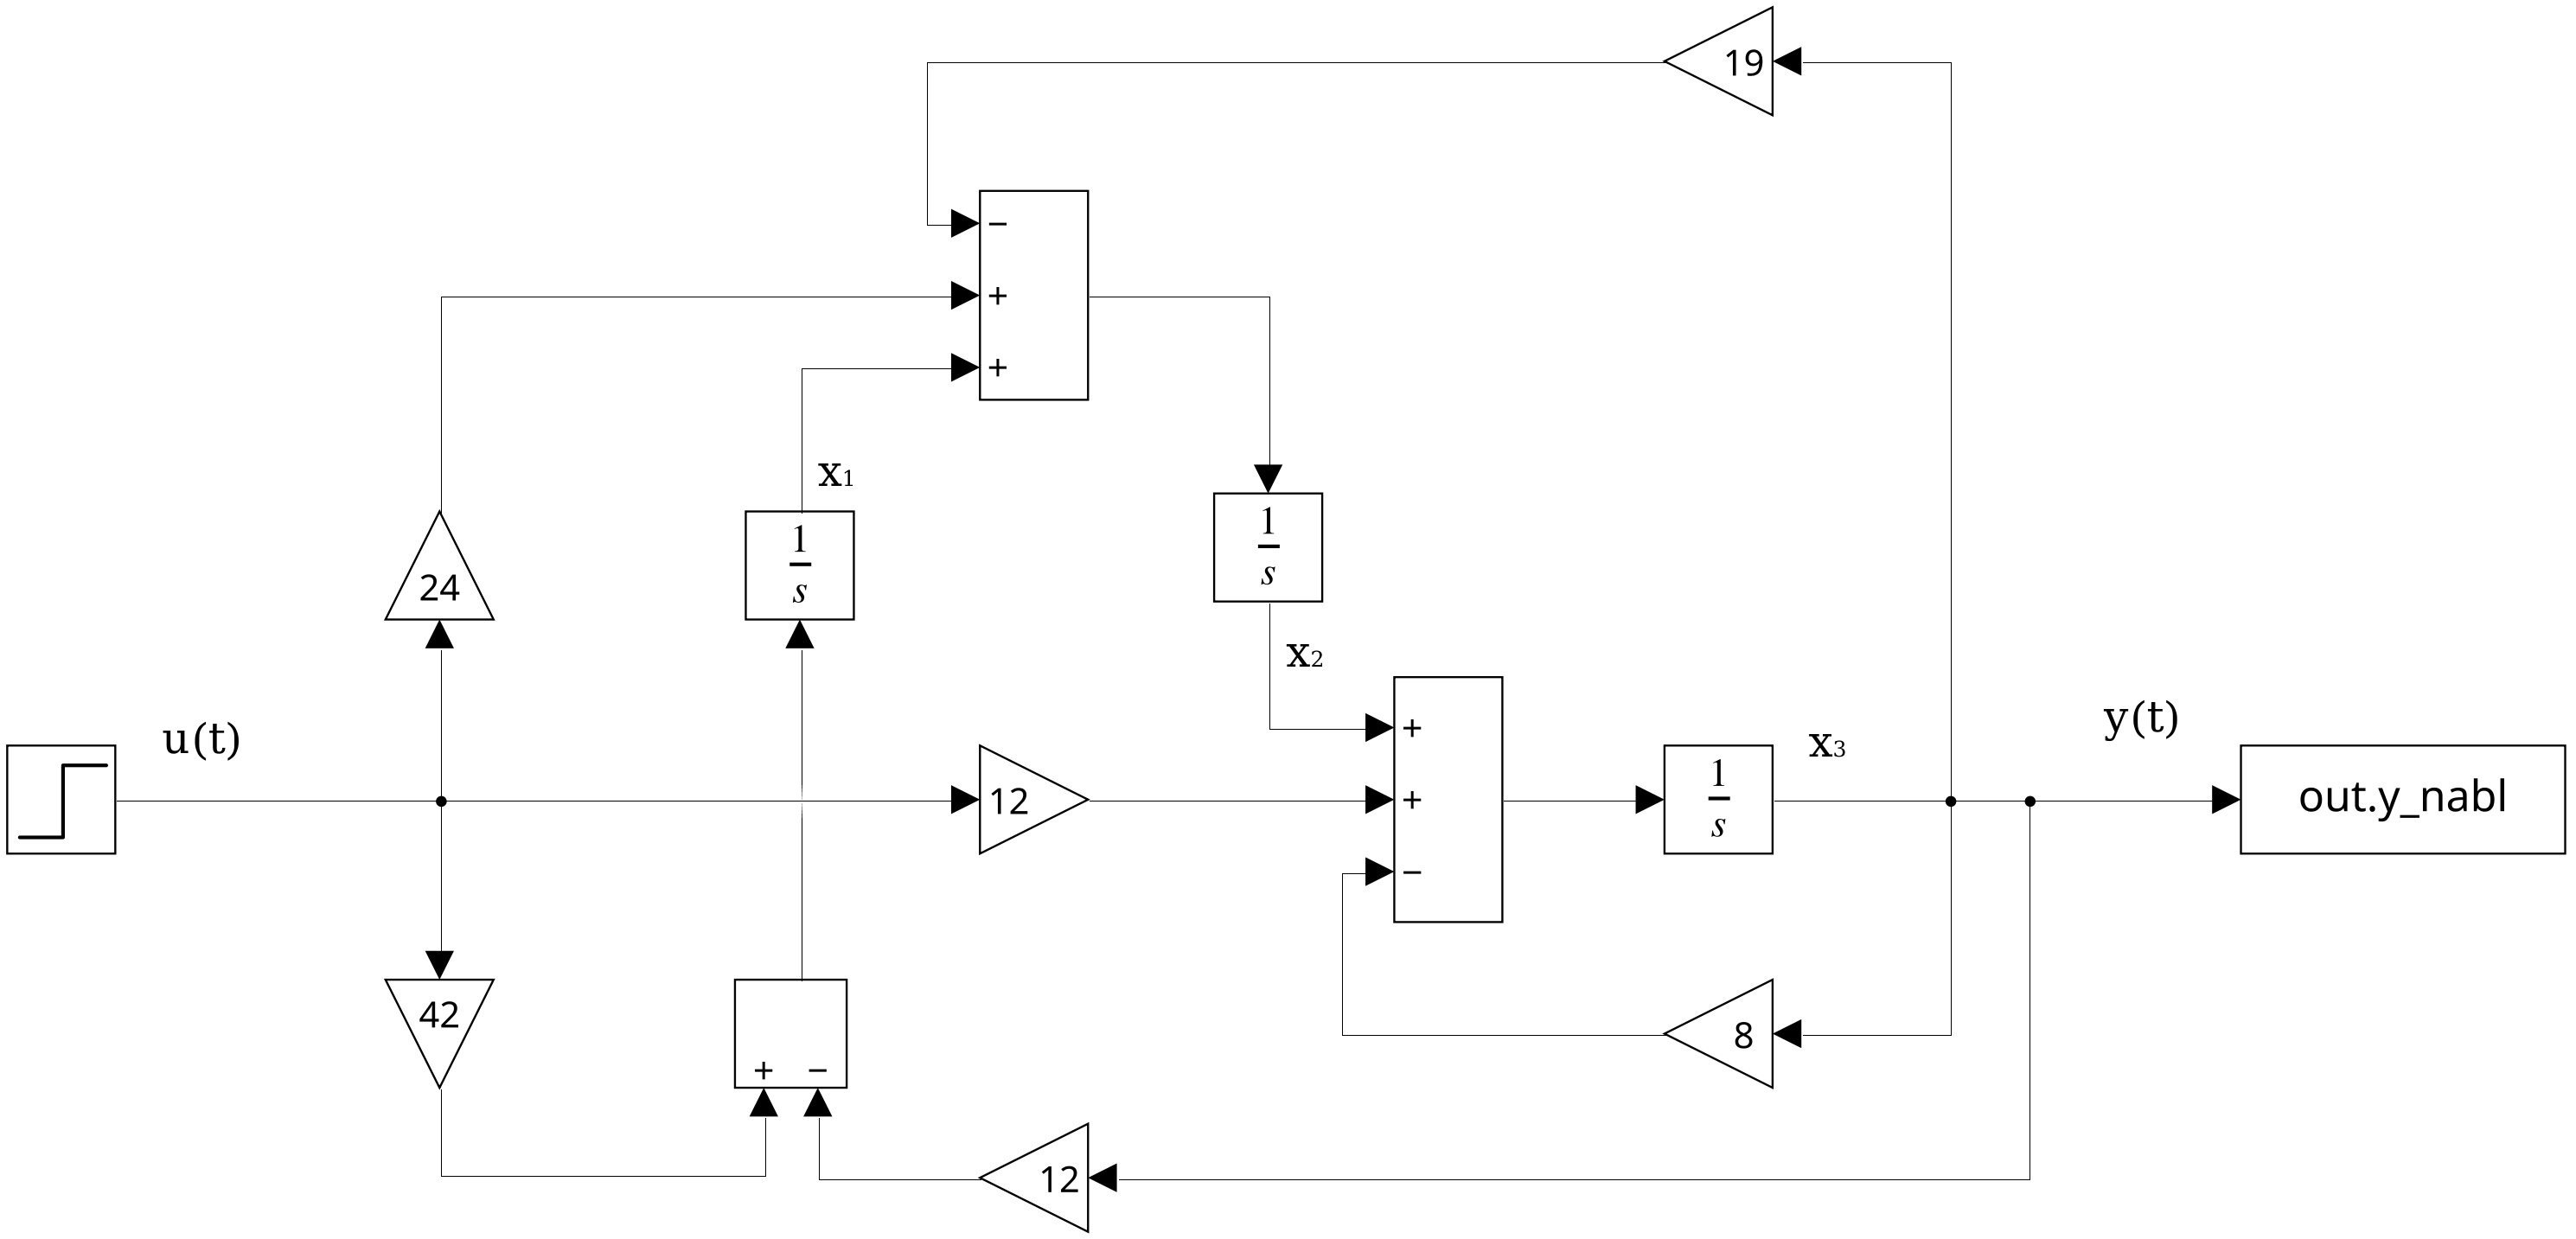
\includegraphics[width=1\textwidth]{../images/task2/model_nabl.png}
		\caption{Сруктурная схема системы в канонической наблюдаемой форме}
	\end{figure}
	
	\subsubsection{Каноническая диагональная форма}
	
	\begin{figure}[H]
		\centering
		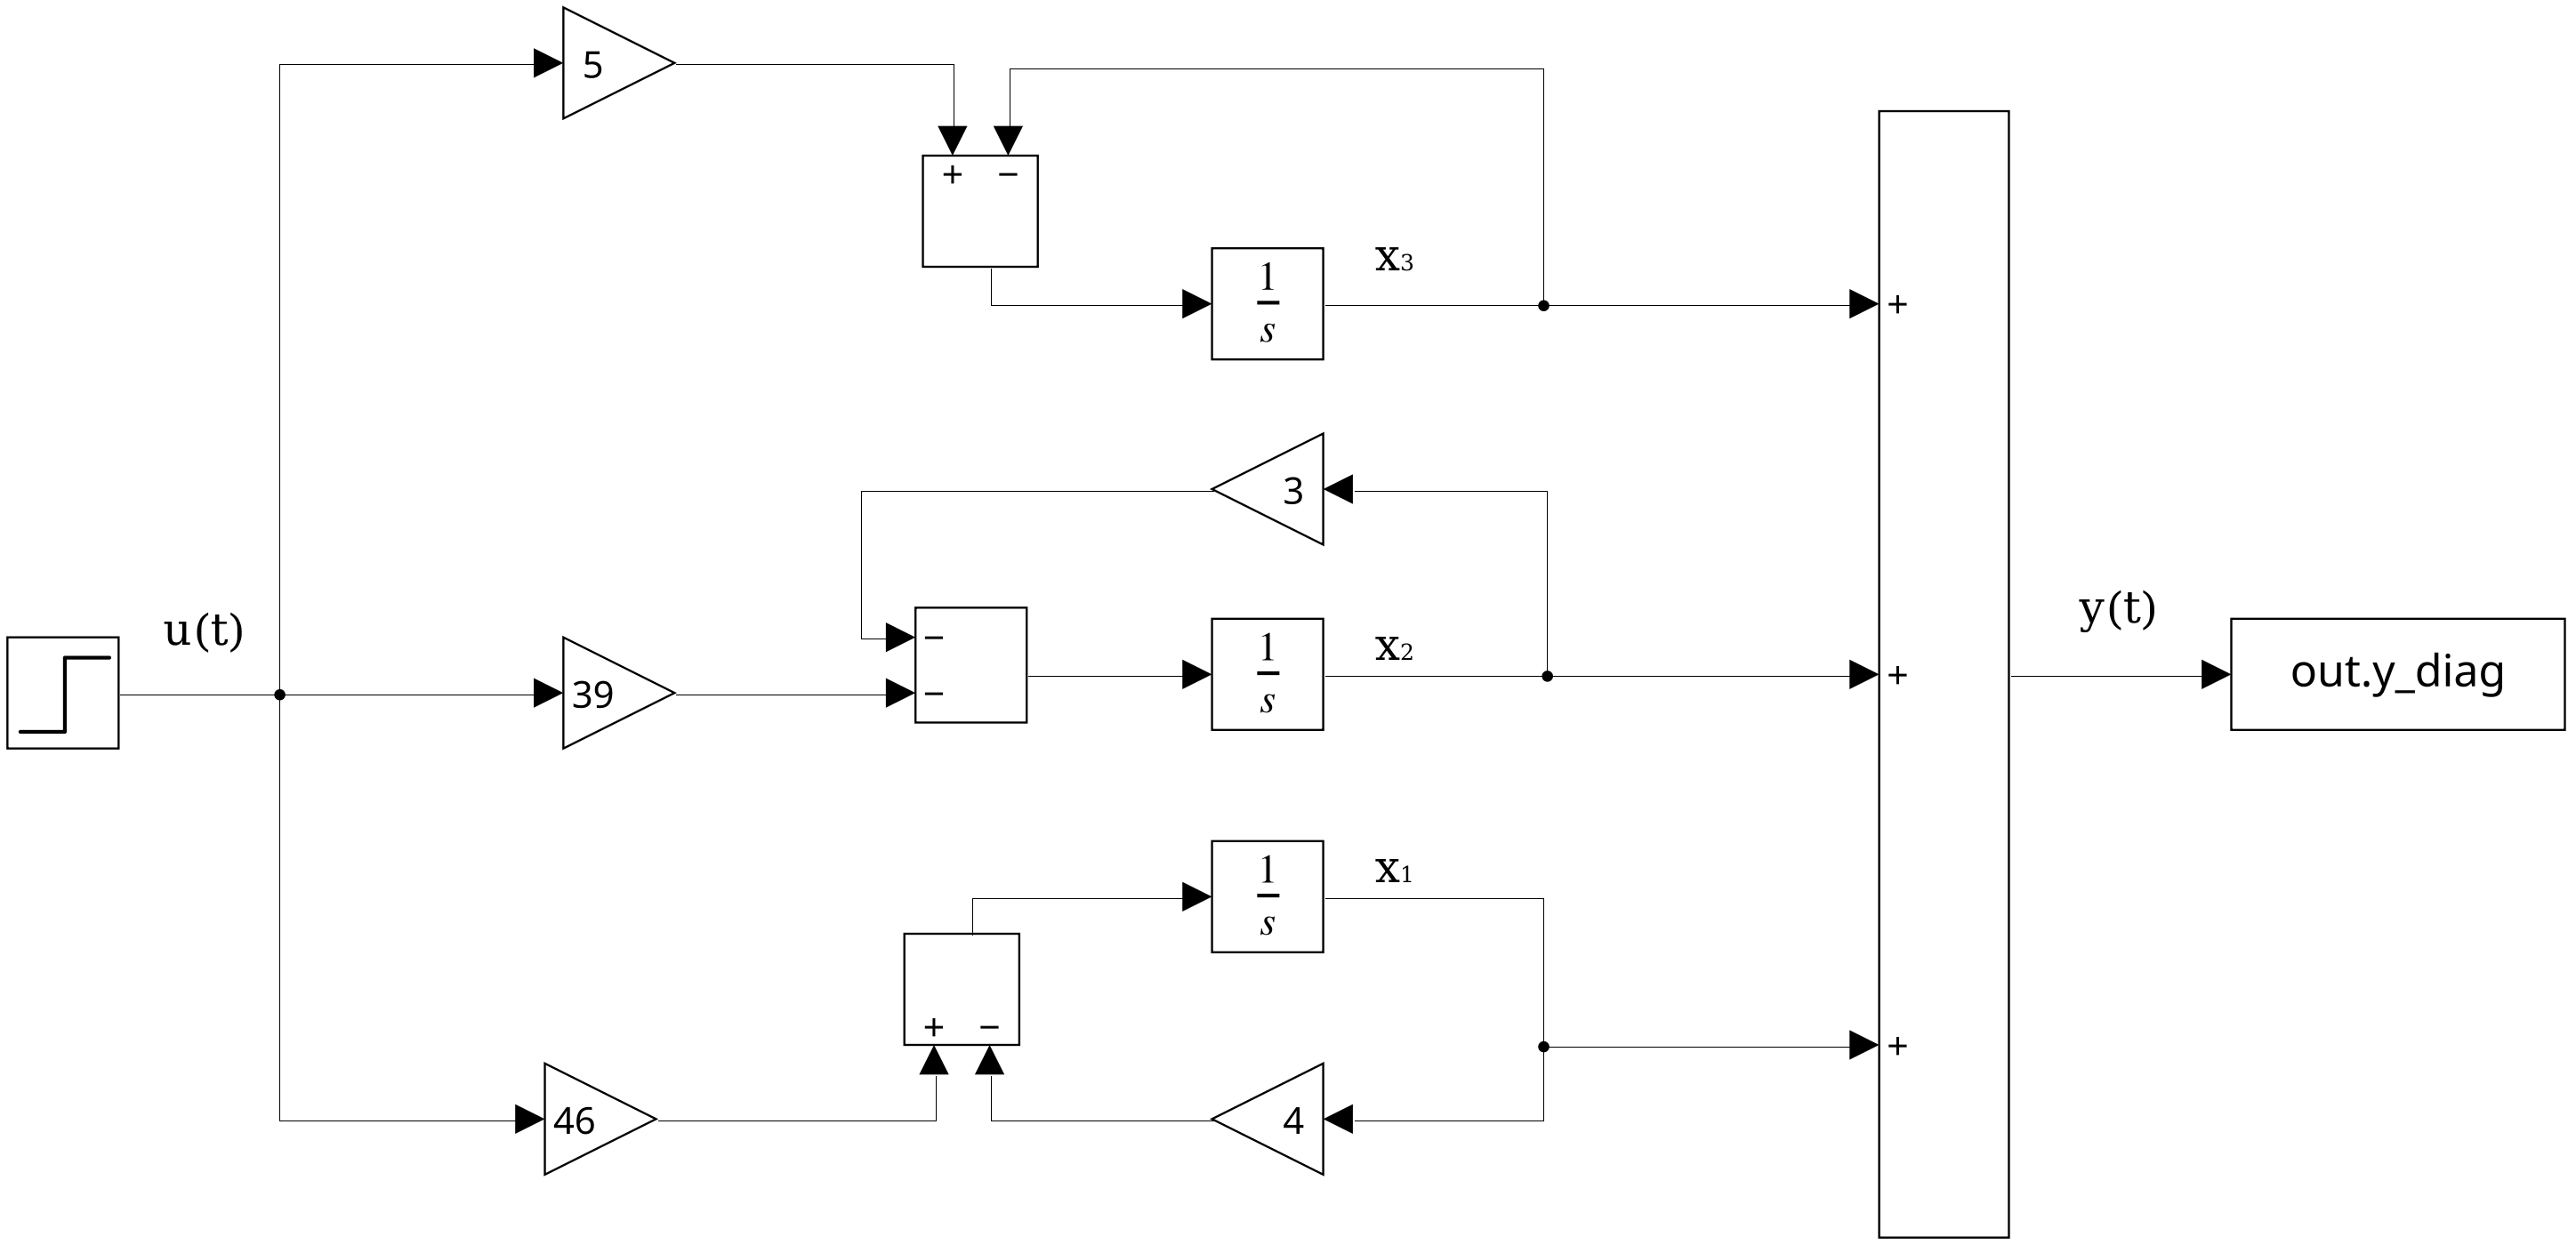
\includegraphics[width=1\textwidth]{../images/task2/model_diag.png}
		\caption{Сруктурная схема системы в канонической диагональной форме}
	\end{figure}
	
	\subsection{Графики входа и выходов}
	
		Подам на вход системы 1 при помощи блока \texttt{Step}. Получится скачок от 0 до единицы в момент времени \(t = 0.0\).
	
	\begin{figure}[H]
		\centering
		
\includegraphics[width=0.9\textwidth]{../images/task1/u.png}
		\caption{Входной сигнал \(u(t)\)}
	\end{figure}
	
	На одном графике отрисую полученные сигналы в канонической управляемой форме \(y_{upr}(t)\), в канонической наблюдаемой форме \(y_{nabl}(t)\), в канонической диагональной форме \(y_{diag}(t)\) и сигнал, полученный при помощи блока \texttt{Transfer FCN} \(y_{Wp}(t)\).
	
	
	\begin{figure}[H]
		\centering
		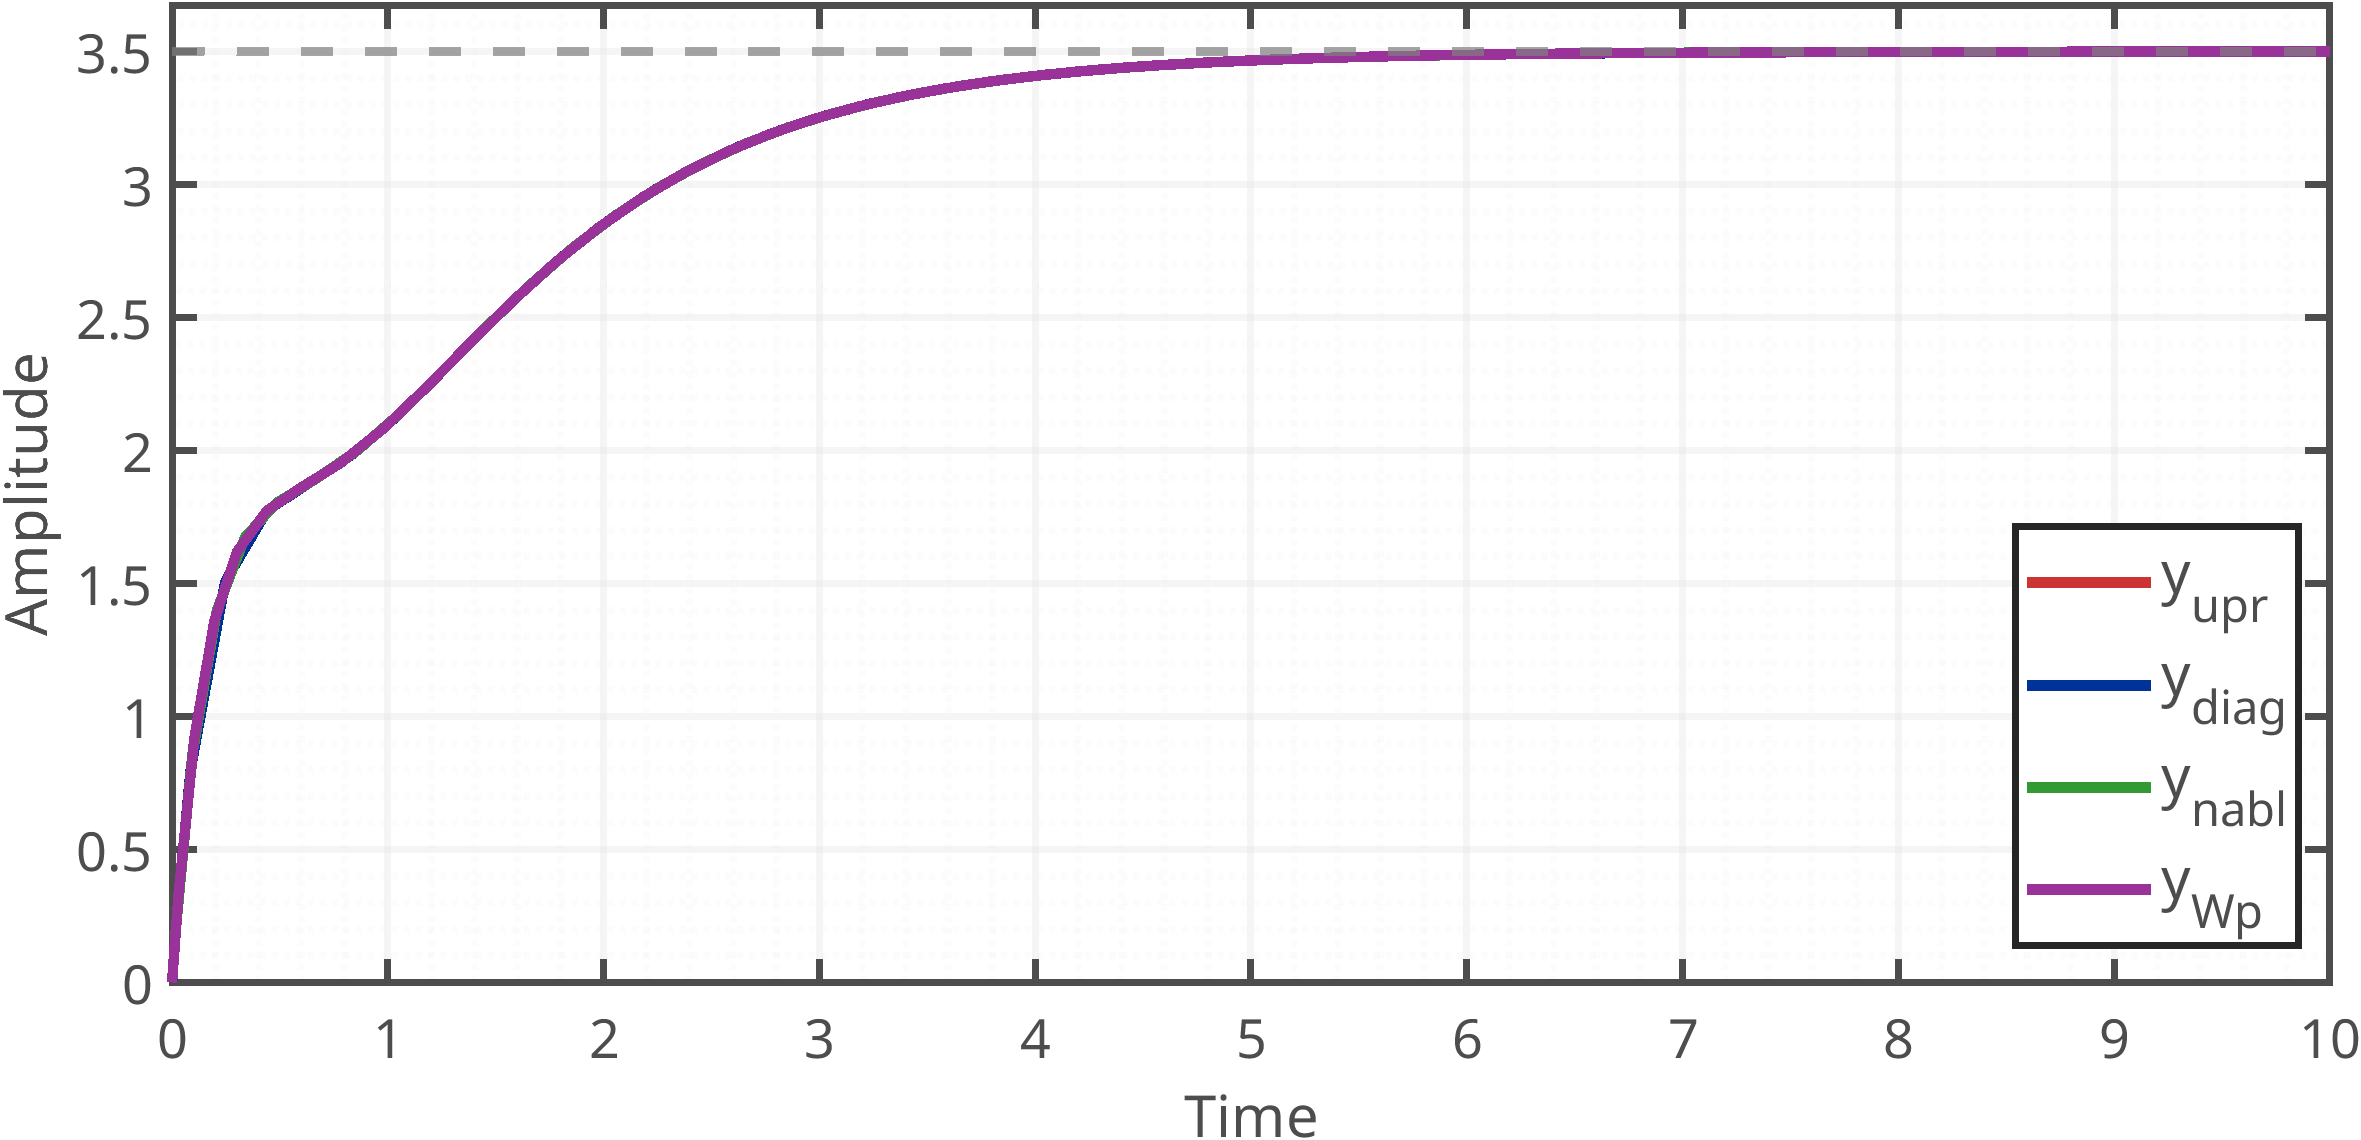
\includegraphics[width=0.9\textwidth]{../images/task2/signals.png}
		\caption{Выходные сигналы \(y_i(t)\)}
	\end{figure}
	
	
	\textbf{Итог:} Все четыре структурные схемы системы демонстрируют идентичное поведение на выходе. Несмотря на различия в математическом представлении и структурной реализации, выходные сигналы полностью совпадают. Это объясняется тем, что различные канонические формы представляют собой замену базиса пространства состояний, при этом входные и выходные характеристики системы остаются неизменными.
	
	
	\newpage
	\section{Задание. Многоканальная система в форме вход-выход}
	
	В этом задании мне нужно:
	
	\begin{itemize}
		
		\item Взять коэффициенты \(a_{ij}(p)\), \(b_{ij}(p)\) из таблицы 2 и рассмотреть систему
		
		\[
		A(p) y(t) = B(p) u(t),
		\quad
		A(p) = \begin{pmatrix}
			a_{11}(p) & a_{12}(p) \\
			a_{21}(p) & a_{22}(p)
		\end{pmatrix},
		\quad
		B(p) = \begin{pmatrix}
			b_{11}(p) & b_{12}(p) \\
			b_{21}(p) & b_{22}(p)
		\end{pmatrix}
		\]
		
		\item Найти передаточную матрицу \(W(p)\).
		
		\item Построить структурную схему системы с блоками, соответствующими передаточным функциям \(W_{ij}(p)\), без разбиения на элементарные операции.
		
		\item Смоделировать систему при входах \(u_1(t) = 1(t)\), \(u_2(t) = \sin(t)\) и нулевых начальных условиях.
		
		\item Представить в отчёте:
		\begin{itemize}
			\item математическую модель (передаточную матрицу),
			\item структурную схему,
			\item графики входов \(u(t)\) и выходов \(y(t)\).
		\end{itemize}
		
	\end{itemize}
	
	\subsection{Математическая модель системы}
	
	Для начала найду передаточную матрицу системы:
	
	\[A(p) y(t) = B(p) u(t)\]
	
	Перенесу \(A(p)\) вправо:
	
	\[
	y(t) = \underbrace{ A^{-1}(p) B(p)}_{\textstyle W(p)} \cdot u(t)
	\]
	
	То есть матрица передаточных функций \(W(p)\) равна:
	
	\[W(p) = A^{-1}(p) B(p)\]
	
	Запишу матрицы \(A\) и \(B\) в соответствии с моим вариантом:
	
	
	\[
	W(p) = 
	\begin{bmatrix}
		p + 11 & p+2 \\
		p + 2 & p + 6
	\end{bmatrix}^{-1}
	\cdot
	\begin{bmatrix}
		9 & 8\\
		1 & 8
	\end{bmatrix}
	\]
	
	Теперь вычислю матрицу \(A^{-1}\). Умножу обратный определитель на транспонированную матрицу алгебраических дополнений:
	
	\[
	A^{-1} = \frac{1}{(p+11) \cdot (p+6) - (p+2)^2} \cdot  
	\begin{bmatrix}
		p + 6 & -(p+2) \\
		-(p+2) & p + 11
	\end{bmatrix}
	= 
	\frac{1}{13p + 62} \cdot  
	\begin{bmatrix}
		p + 6 & -(p+2) \\
		-(p+2) & p + 11
	\end{bmatrix}
	\]
	
	Вычислю передаточную матрицу:
	
	\[
	W(p) = 
	\frac{1}{13p + 62} \cdot  
	\begin{bmatrix}
		p + 6 & -(p+2) \\
		-(p+2) & p + 11
	\end{bmatrix} \cdot  
	\begin{bmatrix}
		9 & 8\\
		1 & 8
	\end{bmatrix} = 
	\frac{1}{13p + 62} \cdot 
	\begin{bmatrix}
		8p+52 & 32\\
		-8p-7 & 72
	\end{bmatrix}
	\]
	
	Итоговая передаточная матрица:
	
	\[
	\renewcommand{\arraystretch}{2.3}
	W(p) =  
	\begin{bmatrix}
		\displaystyle \frac{8p+52}{13p + 62} & \displaystyle \frac{32}{13p + 62} \\
		\displaystyle \frac{-8p-7}{13p + 62} & \displaystyle \frac{72}{13p + 62}
	\end{bmatrix}
	\renewcommand{\arraystretch}{1}
	\]
	
	Запишу математическую модель двухканальной системы в матричном виде:
	
	\[
	\begin{bmatrix}
		y_1(t) \\
		y_2(t)
	\end{bmatrix}
	=
	\renewcommand{\arraystretch}{2.3}
	\begin{bmatrix}
		\displaystyle \frac{8p+52}{13p + 62} & \displaystyle \frac{32}{13p + 62} \\
		\displaystyle \frac{-8p-7}{13p + 62} & \displaystyle \frac{72}{13p + 62}
	\end{bmatrix}
	\renewcommand{\arraystretch}{1}
	\cdot
	\begin{bmatrix}
		u_1(t) \\
		u_2(t)
	\end{bmatrix}
	\]
	
	
	Запишу математическую модель двухканальной системы покомпонентно:
	
	\[
	\begin{cases}
		y_1(t) = \displaystyle \frac{8p+52}{13p + 62} u_1(t) + \frac{32}{13p + 62} u_2(t), \\[12pt]
		y_2(t) = \displaystyle \frac{-8p-7}{13p + 62} u_1(t) + \frac{72}{13p + 62} u_2(t).
	\end{cases}
	\]
	
	Модель описывает взаимовлияние каждого входного сигнала на оба выхода системы через соответствующие передаточные функции.

	\subsection{Структурная схема системы}
	
	 На схеме помимо сигналов показаны передаточные функции:
	
	\[
	W_{11}(p) = \frac{8p+52}{13p + 62}, \quad W_{12}(p) = \frac{32}{13p + 62},
	\]
	
	\[
	W_{21}(p) = \frac{-8p-7}{13p + 62}, \quad W_{22}(p) = \frac{72}{13p + 62}
	\]
	
	Для удобства нарисую два выхода на одной схеме.
	
	\begin{figure}[H]
		\centering
		
\includegraphics[width=1\textwidth]{../images/task3/model.png}
		\caption{Структурная схема двухканальной линейной динамической системы}
	\end{figure}
	
	
	\subsection{Графики входов и выходов}
	
	На одном графике изображу входы системы \(u_1(t) = 1(t)\) и \(u_2(t) = sin(t)\).
	
	\begin{figure}[H]
		\centering
		
\includegraphics[width=0.9\textwidth]{../images/task3/u.png}
		\caption{График входов \(u_1(t)\) и \(u_2(t)\)}
	\end{figure}
	
	Также на одном графике изображу выходы системы \(y_1(t)\) и \(y_2(t)\).
	
	\begin{figure}[H]
		\centering
		
\includegraphics[width=0.9\textwidth]{../images/task3/y.png}
		\caption{График выходов \(y_1(t)\) и \(y_2(t)\)}
	\end{figure}
	
	\textbf{Итог: } В этом задании я получила передаточную матрицу двухканальной системы \( W(p)\), описывающую связь входов и выходов. Построила структурную схему с блоками передаточных функций. Провела моделирование при входах \( u_1(t) = 1(t) \) и \( u_2(t) = \sin(t) \), результаты которого представлены графиками входных и выходных сигналов. 
	
	
	
	
	
	
	
	
	\newpage
	\section{Вывод}
	
	
	\newpage
	\section{Приложение}
	
	
	
	
\end{document}